
\subsection{Обзор современных методов шумоподавления}
Шумоподавление - это активно развивающаяся область, количество методов увеличивается с каждым годом. Поэтому будет удобным, их классифицировать по некоторым признакам. Методы разделяются на то, в каком домене они используются: частотный, пространственный.
К пространственным относятся следующие алгоритмы: Билатеральный, Guided, Non-Local Means, Markov Random Field, Total Variation.
К частотным: BM3D.
Так же разделяются на тип обработки, существуют алгоритмы, которые обрабатывают изображение по пикселям или целыми блоками.
К методом по пиксельной обработки относят: Total Variation.
К блоковым: BM3D, Билатеральный, Guided, Non-Local Means.

\subsection{Билатеральный фильтр}
\subsubsection{Основная идея}
Билатеральный фильтр относится к нелинейным фильтрам, которые сохраняют края и также является некоторым улучшением фильтра гаусса.  При работе фильтра учитывается расстояние до соседнего пикселя и близость значений фильтруемого пикселя и соседнего из окрестности. То есть, влияние пикселя в окрестности некоторого пикселя , для которого вычисляется новое значение будет тем меньше, чем больше разница между интенсивностями и чем больше расстояние между ними\cite{bilateral}.
\subsubsection{Описание}
Нахождения нового значения для пикселя, можно описать следующей формулой:
\begin{equation}
x(u) = \frac{\sum_{p\in N(u)}W_c(\parallel p - u\parallel)W_s(\mid y(u) - y(p)\mid)y(p)}
{\sum_{p\in N(u)}W_c(\parallel p - u\parallel)W_s(\mid y(u) - y(p)\mid)}
\end{equation}
где
\begin{itemize}
\item x(u) - новое значение пикселя
\item p - пиксель исходного изображения
\item u - пиксель, для которого высчитывается новое значение
\item y(u) и y(p) - значения пикселей в исходном изображении
\item N(u) - окрестность пикселя u
\item $W_c$ - весовая функция расстояния с параметров $\sigma_c$ = $exp(\frac{-x^2}{(2\sigma_c^2)})$
\item $W_s$ - весовая функция цвета с параметров $\sigma_s$ = $exp(\frac{-x^2}{(2\sigma_s^2)})$
\end{itemize}

Весовая функция подбирается в зависимости от природы шума. В данном случае выбрана функция Гаусса.

Сохранение краёв на изображении достигается за счёт весовой функции цвета. Если мы считаем новый цвет оказавшись на "темной стороне", т.е. где пиксели принимают низкие значения интенсивности , то как раз "темные" пиксели будут вносить больший вклад, в то время как более "светлые" пиксели, практически не будут влиять на результат. Диапазон интенсивности, который будет влиять на итоговое значение задаётся параметром $\sigma_s$,  при чем зависимость эта прямо пропорциональная.
Параметр $\sigma_c$ определяет радиус окрестности, которая будет влиять на итоговое значение. На практике окрестность пикселя, т.е. её радиус = 2$\sigma_c$.

Рассчитаем сложность алгоритма. Для каждого пикселя, необходимо проверить все пиксели в определенном радиусе. В таком случае сложность алгоритма = $O(nr^2)$, где n - количество пикселей в изображении, r - радиус. 

Одним из главных преимуществ данного фильтра, является его простота, а так же сохранение границ. К сожалению, он так же обладает и рядом недостатков, среди которых:

\begin{itemize}
	\item Долгое время работы
	\item Артефакты на краях цветных изображениях
\end{itemize}

\subsubsection{Результат работы фильтра}
После применения билатерального фильтра c различными параметрами были получены следующие результаты.


\begin{figure}[H]
	\centering
	\subfigure[]{
\includegraphics[scale=0.45]{orig}
		\label{img:orig3}
	}
	\hspace{0.0125ex}
	\subfigure[]{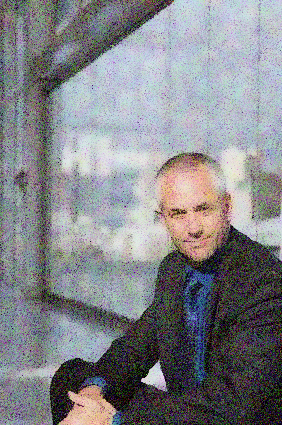
\includegraphics[scale=0.45]{bil1}
		\label{img:bil1}
	}
	\hspace{0.0125ex}
	\subfigure[]{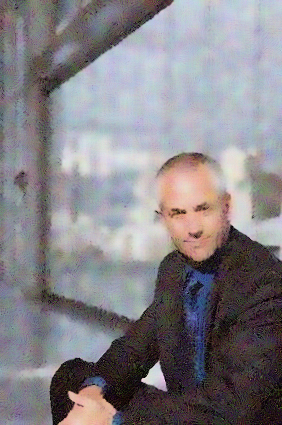
\includegraphics[scale=0.45]{bil2}
		\label{img:bil2}
	}
	\caption{Результаты работы билатерального фильтра: \subref{img:orig3} оригинал; \subref{img:bil1} $radius=11$, $\sigma_s=100$, $\sigma_c=3$; \subref{img:bil2} $radius=11$, $\sigma_s=50$, $\sigma_c=11$}
\end{figure}
Для рис. \ref{img:bil1} PSNR$=28.79$, а для \ref{img:bil2} PSNR$=29.40$.


\subsection{Guided фильтр}
\subsubsection{Основная идея}
Идея заключается в том, что бы найти линейную зависимость определенного блока пикселей исходного изображения с таким же блоком в управляемом изображении. Применяя данную задачу к проблеме шумоподавления, в качестве управляемого изображения используется зашумленное изображение.\cite{He}
\subsubsection{Описание}
Запишем линейную зависимость между пикселем на выходе фильтра и пикселем управляемого изображение в определенном окне следующим образом:
\begin{equation}\label{eq:Guided}
	q_i=a_kI_i+b_k, \forall i \in \omega_k
\end{equation} 
где: 
\begin{itemize}
	\item $q_i$ - итоговое значение пикселя $i$
	\item $I_i$ - значения пикселя $i$ управляемого изображения
	\item $a_k, b_k$ - линейные коэффициенты
	\item $\omega_k$ - окно с центром в пикселе $k$
\end{itemize}
Обычно в качестве окна используют квадрат с радиусом $r$.
Для того, что бы определить линейные коэффициенты рассмотрим уравнение, которое минимизирует разницу между итоговым изображением $q$ и входным изображением $p$. Введем следующую целевую функцию:
\begin{equation}
	E(a_k,b_k) = \sum_{i\in \omega_k}((a_kI_i+b_k)^2+\varepsilon a_k^2)
\end{equation}
Здесь $\varepsilon$ - регуляризационный параметр предотвращающий слишком большое значения $a_k$. Благодаря методу линейной регрессии получим следующие значения для линейных коэффициентов:
\begin{equation}
	a_k=\frac{\frac{1}{|\omega_k|}\sum_{i \in \omega_k}I_ip_i-\mu_k\overline{p}_k}{\sigma_k^2 + \varepsilon}
\end{equation}
\begin{equation}
b_k=\overline{p}_k-a_k\mu_k
\end{equation}
где
\begin{itemize}
	\item $\mu_k$ - среднее значение управляемого изображения $I$ в окне $\omega_k$
	\item $\sigma_k$ - среднеквадратичное отклонение изображеня $I$ в окне $\omega_k$
	\item $|\omega|$ - количество пикселей в окне $\omega_k$ 
	\item $\overline{p_k}$ - среднее значение исходного изображение $I$ в окне $\omega_k$
\end{itemize}
Теперь применим данную модель к целому изображению. Но пиксель $i$ может находится одновременно в нескольких окнах $\omega_k$, поэтому итоговое значения $q_i$ будет отличаться от локального. Простым решением будет взять среднее значение от всех $\omega_k$ в изображении. В конечном итоге получим:
\begin{equation}
	q_i=\frac{1}{|\omega_k|}\sum_{k:i\in \omega_k}(a_kI_i+b_k)\\
	= \overline{a}_kI_i+\overline{b}_k
\end{equation}


Свойства сохранения краев можно объяснить следующим способом, возьмем вспомогательное изображение равное исходному т.е. $I=p$, в таком случае могу быть рассмотрены два крайних случая.
В случае, когда  окно будет гладким, т.е. значения пикселей будут мало отличаться друг от друга, в таком случае параметр $a_k=0$, а $b_k=\overline{p_k}$. 
В противоположном случае, $a_k=1$, а $b_k=0$.
Влияние параметра $\varepsilon$, можно описать следующим образом. Если среднее отклонение $\sigma^2$ меньше, чем $\varepsilon$, то область размывается, в ином случае она остается неизменной.

Главное особенностью данного фильтра является то, что его сложность зависит только от количества пикселей в изображении, т.е. $O(n)$ где $n$ - количество пикселей
\subsubsection{Результат работы фильтра}
\begin{figure}[H]
	\centering
	\subfigure[]{
\includegraphics[scale=0.45]{orig}
		\label{img:orig4}
	}
	\hspace{0.0125ex}
	\subfigure[]{
\includegraphics[scale=0.45]{guided1}
		\label{img:guided1}
	}
	\hspace{0.0125ex}
	\subfigure[]{
\includegraphics[scale=0.45]{guided2}
		\label{img:guided2}
	}
	\caption{Результаты работы guided фильтра: \subref{img:orig4} оригинал; \subref{img:guided1}  $r=5,\varepsilon=0.01$; \subref{img:guided2}$r=9,\varepsilon=0.04$}
	\label{img:guidRes}
\end{figure}
Для рис. \ref{img:bil1} PSNR$=29.27$, а для \ref{img:guided2} PSNR$=25.51$.


\subsection{Non-Local mean фильтр}
\subsubsection{Основная идея}
Обычно, новое значение пикселя берется как некое усредненное значение его соседей. К таким фильтрам относятся: билатеральный фильтр, фильтр скользящего среднего и фильтр Гаусса. Развитием этой идеи стал фильтр NL-mean. Суть его заключается в том, что бы учитывать не только значения интенсивностей пикселей, но так же принимать во внимание схожесть окрестностей пикселей, что позволит наилучшим образом сказываться на сохранении краёв.\cite{non-local}
\subsubsection{Описание}
Идею приведенную выше можно математически описать в следующем виде:
\begin{equation}\label{eq:nl}
	x_i=\sum_j w(i,j)v(j)
\end{equation}
где
\begin{itemize}
\item $x_i$ - итоговое значение пикселя.
\item $w(i,j)$ - весовая функция, которая сравнивает две области изображения, с центром в пикселе i и j
\item $v(j)$ - интенсивность пикселя j
\end{itemize}
Уравнение \ref{eq:nl} указывает зависимость между значением итогового пикселя и всех пикселей исходного, зашумленного изображения:
\begin{equation}
	w(i,j) = \frac{exp(-\frac{\parallel{N(i)-N(j)}\parallel_{2,a}^2}{h})}{\sum_{j \in I}exp(-\frac{\parallel{N(i)-N(j)}\parallel_{2,a}^2}{h})}\
\end{equation}
где
\begin{itemize}
	\item h - параметр указывает степень фильтрации, чем он меньше, тем менее похожие патерны изображения будут влиять на итоговый пиксель
	\item N(i) и N(j) - соседи пикселей i и j
	\item a - стандартное распределение гауссовского фильтра
\end{itemize}
Не трудно заметить, что сложность данного алгоритма $O(n^2(r*2+1))$, это приводит к значительным временным затратам даже для изображений малых размеров.
Для уменьшения сложности вычисления, можно сделать следующие упрощения: можно заранее рассчитать все веса, так как область одного и того же пикселя может использоваться несколько раз, можно уменьшить окно поиска похожих патчей, т.е. теперь похожие патчи буду искаться не во всем изображении, а в некотором окне.  Так же можно сравнивать расстояния не для каждого пикселя, а через один, два и т.д. Тогда сложность будет= $O(n*N*(r*2+1))$, где N размер большого окна.
\subsubsection{Результат работы фильтра}
\begin{figure}[H]
	\centering
	\subfigure[]{
\includegraphics[scale=0.45]{orig}
		\label{img:orig6}
	}
	\hspace{0.0125ex}
	\subfigure[]{
\includegraphics[scale=0.45]{nl1}
		\label{img:nl1}
	}
	\hspace{0.0125ex}
	\subfigure[]{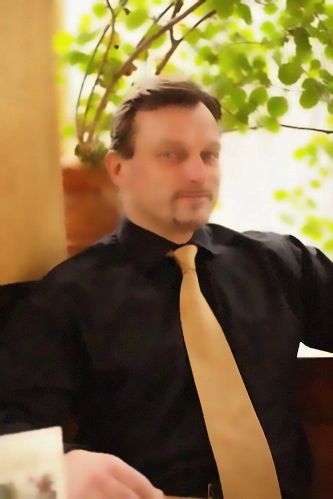
\includegraphics[scale=0.45]{nl2}
		\label{img:nl2}
	}
	\caption{Результаты работы Non-Local mean фильтра: \subref{img:orig6} оригинал; \subref{img:nl1}  Размер шаблона$=3$, радиус поиска$=7$, $h=30$; \subref{img:nl2} Размер шаблона$=3$, радиус поиска$=11$, $h=30$}
	\label{img:nlRes}
\end{figure}
Для рис. \ref{img:nl1} PSNR$=26.29$, а для \ref{img:nl2} PSNR$=25.03$.

\subsection{BM3D}
Фильтр BM3D можно считать более лучшей версией алгоритма Non-Local mean. В нём так же одним из ключевых моментов является
усреднение значений посредством поиска похожих блоков. В алгоритме можно выделить два основных шага. Каждый шаг в свою очередь разбивается на 3 этапа. Первый этап называется группировка ($grouping$), в котором для каждого патча (часть изображения фиксированного размера), отбираются другие похожие патчи. Вторым этапом является совместная ($collaborative$) фильтрация. Третьим этапом является агрегация, где для каждого пикселя вычисляется новое значение, с учетом того, что данный пиксель мог находится в различных патчах\cite{Hasan2018}.
%from https://www.researchgate.net/figure/BM3D-Block-Diagram-Dabov-et-al-2007c_fig1_301721957
\begin{figure}[H]
	\center{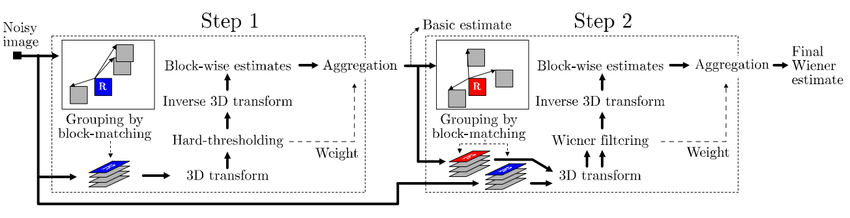
\includegraphics[scale=0.5]{bm3dCircuit.png}}
	\caption{Схема алгоритма BM3D\cite{bm3dCircuit}}
\end{figure}
Далее патчем будет обозначаться часть исходного изображения с фиксированным размером.
\subsubsection{Оценка дисперсии}
Качество работы алгоритма зависит от дисперсии входного изображения. Поэтому для корректной работы алгоритма необходимо правильно оценивать дисперсию.

Для этого используется следующая метрика - MAD (median absolute deviation)\cite{mad}. Выглядит она следующим образом:
\begin{equation}
	\sigma = k * MAD
\end{equation}
где
\begin{itemize}
	\item $\sigma$ - дисперсия
	\item $MAD$ - медианное абсолютное отклонение
	\item $k$ - константа, которая зависит от распределения. В случае нормального распределения $k=1.4826$%вставить. 
	
\end{itemize}
\subsubsection{Первый шаг}
\paragraph{Группировка}\

Всё изображение разбивается на патчи (блоки), которые имеют размером - $N_{ht}^{Psize}$.  Далее для каждого патча, обозначим его $P$, производятся следующие действия. В окне размера - $N_{ht}^Wsize$, в котором центром является $P$, с шагом - $N_{ht}^{Sstep}$ ищутся похожие блоки  \ref{eq:l2bm3d}:
\begin{equation}\label{eq:l2bm3d}
	G_{ht}(P) = \left\{Q | d_{ht}(Q,P) \leq h_{ht}\right\}
\end{equation}
где
\begin{itemize}
	\item $G_{ht}(P)$ - множество блоков схожих с P
	\item Q - один из блоков в окне
	\item $d_{ht}(Q,P) = \frac{\parallel\gamma_{\lambda_{ht}^{2D}}(P)-\gamma_{\lambda_{ht}^{2D}}(Q)\parallel_2^2}{(N_{ht}^{Psize})^2}$
	\item $\gamma_{\lambda}(x) = \begin{cases}0 &|x| \leq \lambda\\ x & |x| > \lambda\end{cases}$ - жесткая пороговая фильтрация 
	\item $\lambda_{ht}^{2d}$ - для низких значений шума $\sigma < 40$ обычно равняется нулю, подробнее \cite{dabov}
	\item $\sigma^2$ -  дисперсия шума
	\item $h_{ht}$ - порог, для того, что бы считать два блока похожими.
\end{itemize}
Максимальное количество подходящих блоков так же ограничивают, за это отвечает параметр - $N_{ht}^{Pmax}$. Найденные блоки объединяются в 3D-блок, далее обозначаемый $G_{ht}^{3D}(P)$,в котором блоки располагаются по мере уменьшения схожести.

\paragraph{Совместная фильтрация}\

К $G_{ht}^{3D}(P)$ применяется 3D преобразование - $r_{ht}^{3D}$, трансформирующие его в частотную область, после применяется жесткая пороговая фильтрация $\gamma_{\lambda_{ht}^{3D}}$. После данных операций происходит обратное 3D преобразование - $r_{ht}^{3D^{-1}}$ . Данные действия описываются следующей формулой:
\begin{equation}
G_{ht}^{3D'}(P) = r_{ht}^{3D^{-1}}(\gamma_{\lambda_{ht}^{3D}}(r_{ht}^{3D}(G_{ht}^{3D}(P))))
\end{equation}

\paragraph{Агрегация}\

Теперь для каждого пикселя в изображении, необходимо рассчитать новое значение. При этом нужно учесть, что пиксель мог находится в нескольких $G_{ht}^{3D'}$. Итоговая формула следующая:
\begin{equation}
	y^{basic}(x) = \frac{\sum\limits_Pw_p^{hard}\sum\limits_{Q \in G_{ht}^{3D'}(P)}\chi_Q(x)u_{P,Q}(x)}{\sum\limits_Pw_p^{ht}\sum\limits_{Q \in G_{ht}^{3D'}(P)}\chi_Q(x)}
\end{equation}
где
\begin{itemize}
	\item $y^{basic}(x)$ - значение пикселя после первого шага 
	\item $w_p^{ht}  = \begin{cases}(N_p^{hard})^{-1} & N_p^{hard} \geq 1\\ 1 & N_p^{hard} < 1 \lambda\end{cases}$
	\item $N_p^{hard}$ - количество ненулевых пикселей после $\gamma_{\lambda_{ht}^{3D}}(r_{ht}^{3D}(G_{3D}(P))$
	\item $\chi_Q(x)$ - равняется 1, если $x\in Q$
\end{itemize}

\subsubsection{Второй шаг}
На основе $y^{basic}$ можно получить более лучшее шумоподавления, применяя фильтр Винера. Патч, для которого произведены дальнейшие действия обозначим $P^{basic}$
\paragraph{Группировка}\

Будем считать, что количество шума после первого шага сведенно к минимуму. Определим формулу, для поиска подходящих блоков на втором шаге:
\begin{equation}
	G_{wie}(P^{basic}) = \left\{Q | d_{wie}(Q,P^{basic}) \leq h_{wie}\right\}
\end{equation}
где
\begin{itemize}
	\item $G_{wie}(P^{basic})$ - множество блоков схожих с $P^{basic}$
	\item Q - один из блоков в окне
	\item $d_{wie}(Q,P^{basic}) = \frac{\parallel P^{basic} - Q\parallel_2^2}{(N_{ht}^{Psize})^2}$
	\item $h_{wie}$ - порог, для того, что бы считать два блока похожими.
\end{itemize}

\paragraph{Совместная фильтрация}
Объединим блоки найденные на этапе группировка второго шага в $G_{wie}^{3D}(P^{basic})$. Затем применим 3D преобразование - - $r_{wie}^{3D}$, как в первом шаге. Применим фильтр Винера: поэлементно умножим $G_{wie}^{3D}(P^{basic})$ на коэффициент сжатия Винера - $w_P$. После, применим обратное 3D преобразование - $r_{ht}^{3D^{-1}}$. Опишем эти действия следующей формулой:
\begin{equation}
G_{wie}^{3D'}(P^{basic}) = r_{wie}^{3D^{-1}}(w_P \cdot r_{wie}^{3D}(G_{wie}^{3D}(P)))
\end{equation}
где
\begin{itemize}
\item  $w_P = \frac{|r_{wie}^{3D}(G_{wie}^{3D}(P^{basic})|^2}{|r_{wie}^{3D}(G_{wie}^{3D}(P^{basic})|^2 + \sigma} $
\end{itemize}
\paragraph{Агрегация}\

Агрегация на втором шаге проводится по следующей формуле:
\begin{equation}
y(x) = \frac{\sum\limits_Pw_p^{wie}\sum\limits_{Q \in G_{wie}^{3D'}(P)}\chi_Q(x)u_{P,Q}(x)}{\sum\limits_Pw_p^{wie}\sum\limits_{Q \in G_{wie}^{3D'}(P)}\chi_Q(x)}
\end{equation}
где
\begin{itemize}
	\item $y(x)$ - итоговое значение пикселя
	\item $w_P^{wie}  = \parallel w_P \parallel_2^{-2}$ 
\end{itemize}

\subsubsection{Оптимальные параметры}
Согласно \cite{bm3d}, оптимальными параметрами будут следующие:

\begin{tabular}{|c|c|c|}
	\hline
	Обозначение параметра & $\sigma \leq 40$ & $\sigma > 40$\\
	\hline
	$N_{ht}^{Pmax}$ & 16 & 16 \\
	\hline
	$N_{wie}^{Pmax}$ & 32 & 32 \\
	\hline
	$N_{ht}^{Psize}$ & 8 & 8 \\
	\hline
	$N_{wie}^{Psize}$ & 8 & 8 \\
	\hline
	$\lambda_{ht}$ & 2.7 & 2.7 \\
	\hline
	$h_{ht}$ & 2500 & 5000 \\
	\hline
	$h_{wie}$ & 400 & 3500 \\ 
	\hline
	
\end{tabular}
\subsubsection{Результат работы фильтра}

\begin{figure}[H]
	\centering
	\subfigure[]{
\includegraphics[scale=0.45]{orig}
		\label{img:orig7}
	}
	\hspace{0.0125ex}
	\subfigure[]{
\includegraphics[scale=0.45]{bm3d}
		\label{img:bm3d}
	}
	\caption{Результаты работы BM3D фильтра: \subref{img:orig7} оригинал; \subref{img:bm3d} после BM3D фильтра}
	\label{img:bm3dRes}
\end{figure}
Для рис. \ref{img:bm3d} PSNR$=32.18$.

\subsection{Total Variation фильтр}
\subsubsection{Основаная идея}
Для описании основной идее потребуются определить вариацию функции (total variation) - показывает насколько сильно изменился сигнал между своими значениями. Применяя это описания для одномерного дискретного конечного сигнала $x$ длиной $N$ получим: 
\begin{equation}\label{eq:TV}
TV(x)=\sum_{n=2}^N|x(n) - x(n-2)|
\end{equation}
Так же вариацию функции удобно описать в матричном виде:
\begin{equation}\label{eq:TV:m}
	TV(x) = \parallel xD\parallel_1
\end{equation}
где $\parallel  \cdot  \parallel_1$ - $\ell_1$  норма а,
\begin{equation}\label{eq:TV:matrix}
D = \left[
\begin{array}{ccccc}
-1 & 1 & & & \\
 & -1 &  1& & \\
 & & \ddots & & \\
 &  &  & -1  & 1 
\end{array}
\right]
\end{equation}
матрица размером $(N-1)\times N$
Предполагается, что на бесшумном изображении вариация функции меньше, чем на зашумленном, поэтому данную функцию можно использовать в качестве регуляризационного члена целевой функции, которая будет определена далее.
\subsubsection{Описание}
Необходимо найти неискаженное шумом изображение $x$ с помощью зашумленного изображения $y$. Для этого введем целевую функцию, где регуляризационным членом будет выражение \ref{eq:TV:m}:
\begin{equation}
J(x) = \lambda \parallel D x \parallel_1+\parallel x-y\parallel_2^2
\end{equation}
где:
\begin{itemize}
	\item x - итоговое изображение, представленное в виде матрицы
	\item D - трехмерная матрица определенная в \ref{eq:TV:matrix}
	\item $\lambda$ - регуляризационный параметр 
	\item y - зашумленное изображение, представленное в виде матрицы 
\end{itemize}
Соотвественно оптимальное значение можно обозначить следующим образом:
\begin{equation}
J_* = \min_x \parallel y-x\parallel^2_2 + \lambda\parallel Dx\parallel_1
\end{equation}
Нахождения оптимального значения является сложной задачей, из-за того что $\ell_1$ норма не дифференцируема. Рассмотрим задачу как двойственную.
Для этого представим $\ell_1$ норму в следующей форме:
\begin{equation}
	\parallel x \parallel_1 = \max_{|z| \le 1}z^tx
\end{equation}
Таким образом мы получим:
\begin{equation}\label{eq:TV:2}
	J_x=\min_x\max_{|z| \le 1}\parallel y-x \parallel_2^2+\lambda z^t Dx
\end{equation}
Описание вывода решения двойственной задачи \ref{eq:TV:2} будет опущенно, так как оно не входит в рамки данной ВКР. Результатом является итерационный алгоритм, который выглядит следующим образом:
\begin{fleqns}
\begin{gather*}
\;\;x^{(i+1)}=y-D^tz^{(i)} \\
\;\;z^{(i+1)}=clip(z^{(i)} + \frac{1}{\alpha}Dx^{(i+1)}, \frac{\lambda}{2})\\
for  \;i \ge 0 \; with z^{(0)}=0\; and\;a\ge maxeig(A,A')
\end{gather*}
\end{fleqns}


\subsubsection{Результат работы фильтра}


\begin{figure}[H]
	\centering
	\subfigure[]{
\includegraphics[scale=0.45]{orig}
		\label{img:orig8}
	}
	\hspace{0.0125ex}
	\subfigure[]{
\includegraphics[scale=0.45]{tv1.png}
		\label{img:tv1}
	}
	\hspace{0.0125ex}
	\subfigure[]{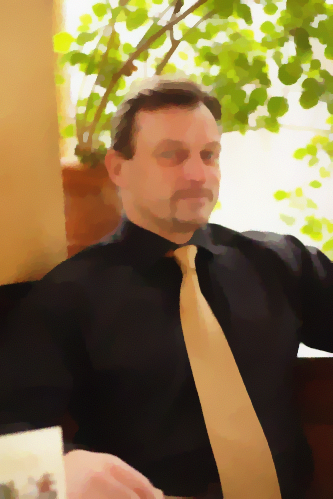
\includegraphics[scale=0.45]{tv2.png}
		\label{img:tv2}
	}
	\caption{Результаты работы фильтра на основе вариации функции с различными регуляризационными параметрам: \subref{img:orig8} оригинал; \subref{img:tv1} $\lambda=1$; \subref{img:tv1} $\lambda=0.6$}
\end{figure}
Для рис. \ref{img:tv1} PSNR$=27.93$, а для \ref{img:tv2} PSNR$=24.95$.

% во всех главах
\subsection{Выводы по разделу}
В данном разделе была поставлена задача шумоподавления, были рассмотрены самые простые методы обработки изображений и выявлены их недостатки. Так же были классифицированны некоторые продвинутые методы шумоподавления. Были описаны основные идеи каждого фильтра и их математическое описание.